\documentclass[10pt,a4paper,twocolumn]{article}
% Shared preamble for the synthetic Turkish corpus (compiled with tectonic).
\usepackage{iftex}
\ifXeTeX
  \usepackage{fontspec} % Latin Modern OpenType, proper ToUnicode for Turkish letters
\else
  \usepackage[T1]{fontenc}
  \usepackage[utf8]{inputenc}
  \usepackage{lmodern}
\fi
\usepackage[turkish,shorthands=off]{babel}
\usepackage{amsmath,amssymb}
\usepackage{graphicx}
\usepackage{xcolor}
\usepackage{tikz}
\usepackage{booktabs}
\usepackage{hyperref}
\hypersetup{colorlinks=true,linkcolor=blue!50!black,urlcolor=blue!50!black,citecolor=green!40!black}
\newcommand{\paragrafA}{Makine çevirisi sistemleri son on yılda büyük bir gelişme göstermiştir. Özellikle sinir ağı tabanlı yöntemler, kelime düzeyinde değil tümce düzeyinde bağlamı dikkate alarak daha akıcı çeviriler üretmektedir. Bununla birlikte akademik metinlerde terimlerin tutarlı biçimde çevrilmesi, kesinlik derecesinin korunması ve sayısal değerlerin değiştirilmemesi hâlâ önemli sorunlar arasında yer almaktadır.}
\newcommand{\paragrafB}{Bu çalışmada 2019–2023 yılları arasında yayımlanmış 412 makaleden oluşan bir derlem kullanılmıştır. Her makale için özet, giriş ve sonuç bölümleri ayrı ayrı değerlendirilmiş; toplam 18.640 tümce iki bağımsız uzman tarafından incelenmiştir. Uzmanlar arasındaki uyum katsayısı $\kappa = 0{,}81$ olarak hesaplanmıştır.}
\newcommand{\paragrafC}{Bulgular, uzun ve iç içe geçmiş tümcelerde terim tutarlılığının belirgin biçimde azaldığını göstermektedir. Ortalama terim tutarlılığı \%87,4 olarak ölçülmüş; ancak kırk sözcükten uzun tümcelerde bu oran \%71,2'ye düşmüştür. Bu fark istatistiksel olarak anlamlıdır ($p < 0{,}01$).}

\usepackage[margin=1.8cm,columnsep=0.6cm]{geometry}
\begin{document}
\twocolumn[{\centering{\LARGE\bfseries İki Sütunlu Düzende Paragraf Zincirleri}\par\vspace{0.5em}{\large Zeynep Kaya}\par\vspace{1.5em}}]
\section{Giriş}
\paragrafA\ \paragrafB\ \paragrafC\ \paragrafA\ \paragrafB
\section{İlgili Çalışmalar}
\paragrafC\ \paragrafA\ \paragrafB\ \paragrafC\ \paragrafA\ \paragrafB\ \paragrafC
\begin{figure}[t]
\centering
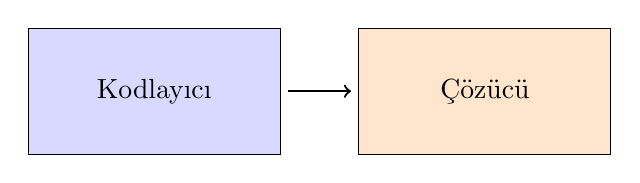
\begin{tikzpicture}
\draw[fill=blue!15] (0,0) rectangle (3.2,1.6);
\node at (1.6,0.8) {Kodlayıcı};
\draw[->,thick] (3.3,0.8) -- (4.1,0.8);
\draw[fill=orange!20] (4.2,0) rectangle (7.4,1.6);
\node at (5.8,0.8) {Çözücü};
\end{tikzpicture}
\caption{Kodlayıcı–çözücü mimarisinin şematik gösterimi.}
\end{figure}
\section{Yöntem}
\paragrafB\ \paragrafA\ \paragrafC\ \paragrafB\ \paragrafA\ \paragrafC\ \paragrafB\ \paragrafA
\begin{table}[b]
\centering
\caption{Tümce uzunluğuna göre terim tutarlılığı.}
\begin{tabular}{lrr}
\toprule
Uzunluk & Tümce & Tutarlılık (\%) \\
\midrule
Kısa & 9.120 & 87,4 \\
Orta & 6.310 & 80,9 \\
Uzun & 3.210 & 71,2 \\
\bottomrule
\end{tabular}
\end{table}
\section{Sonuç}
\paragrafC\ \paragrafA\ \paragrafB\ \paragrafC\ \paragrafA\ \paragrafB\ \paragrafC\ \paragrafA\ \paragrafB
\end{document}
